\begin{exercise}
      {ID-75006fd98ddb3301d1bc23ff2e2161e89c1f37e3}
      {Begründung}
  \ifproblem\problem\par
    Begründe mithilfe der Abbildung, warum der Satz des Pythagoras richtig ist.
    \begin{center}
      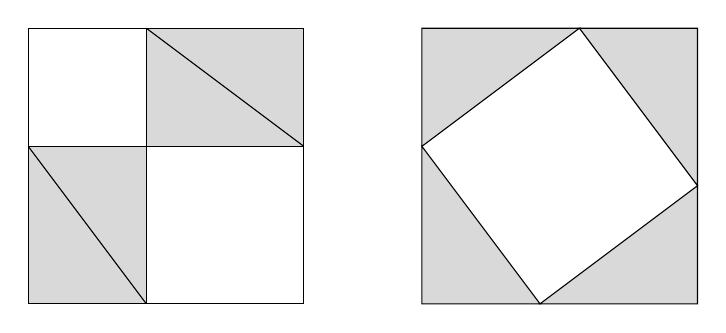
\begin{tikzpicture}[scale=0.5]
        \begin{scope}
          \fill[fill=black!15!white] (0, 0) rectangle (3, 4);
          \fill[fill=black!15!white] (3, 4) rectangle (7, 7);
          \draw (0, 0) rectangle (7, 7);
          \draw (3, 0) -- (3, 7);
          \draw (0, 4) -- (7, 4);
          \draw (3, 7) -- (7, 4);
          \draw (0, 4) -- (3, 0);
        \end{scope}
        \begin{scope}[xshift=10cm]
          \filldraw[fill=black!15!white] (0, 0) -- (3, 0) -- (0, 4) -- cycle;
          \filldraw[fill=black!15!white] (0, 4) -- (4, 7) -- (0, 7) -- cycle;
          \filldraw[fill=black!15!white] (3, 0) -- (7, 0) -- (7, 3) -- cycle;
          \filldraw[fill=black!15!white] (7, 3) -- (7, 7) -- (4, 7) -- cycle;
        \end{scope}
      \end{tikzpicture}
    \end{center}
  \fi
  %\ifoutline\outline\par
  %\fi
  %\ifoutcome\outcome\par
  %\fi
\end{exercise}
